% \documentclass{IEEEtran}
\documentclass{article}
\title{A Three-Day Exploration of Eastern Washington (draft)}

% Packages
\usepackage[utf8]{inputenc} % UTF-8 encoding
\usepackage[T1]{fontenc} % Font encoding
\usepackage{graphicx} % For including images
\usepackage{pdflscape} % for landscape environment
\usepackage{hyperref} % For hyperlinks
\usepackage{tikz} % for drawing diagrams
\usetikzlibrary{chains, positioning}
\usepackage{float}
\usepackage{geometry}
\usepackage{array}
\usepackage[dvipsnames]{xcolor}
\usepackage[normalem]{ulem} % For \sout (strikethrough)

% Hyperlinks
\newcommand{\WildHorseRenewableEnergyCenter}{\href{https://maps.app.goo.gl/HyvLjvWAAMydgWg18}{Wild Horse Renewable Energy Center}}
\newcommand{\WildHorseMonument}{\href{https://maps.app.goo.gl/RgAQq2vTrCyx1wKb7}{Wild Horse Monument}}
\newcommand{\ScenicOverlookOftheColumbiaRiver}{\href{https://maps.app.goo.gl/EnTs5yzFyGQKeNPo8}{Scenic Overlook of the Columbia River}}
\newcommand{\PalouseFallsStatePark}{\href{https://maps.app.goo.gl/9GDtt9Re3oMoWs216}{Palouse Falls State Park}}
\newcommand{\Pullman}{\href{https://google.com}{Pullman}}
\newcommand{\KamiakButteCountryPark}{\href{https://maps.app.goo.gl/1tkTZRiLE7eipXeE9}{Kamiak Butte Country Park}}
\newcommand{\SteptoeButteStatePark}{\href{https://maps.app.goo.gl/6vj1gx25XB5dEsUW8}{Steptoe Butte State Park}}
\newcommand{\Spokane}{\href{https://google.com}{Spokane}}
\newcommand{\DryFallsVisitorCenter}{\href{https://maps.app.goo.gl/ikKJMB3SaaTAfcYT9}{Dry Falls Visitor Center}}
\newcommand{\LakeChelanStatePark}{\href{https://maps.app.goo.gl/SG8UQnPoWd1ubnXq7}{\sout{Lake Chelan State Park}}}
\newcommand{\WildHorseMonumentWebsite}{\href{https://www.wta.org/go-hiking/hikes/wild-horses-monument}{Wild Horse Monument Website}}

% Define colors.
% \definecolor{mycolor}{RGB}{0,191,255} % Define custom RGB color
\definecolor{mycolor}{RGB}{150,150,150} % Define custom RGB color
\definecolor{locationBg}{RGB}{150,150,150} % Define custom RGB color
\definecolor{dayOneColor}{RGB}{71,204,211} % Define custom RGB color
\definecolor{dayTwoColor}{RGB}{110,64,171} % Define custom RGB color
\definecolor{dayThreeColor}{RGB}{56,151,216} % Define custom RGB color

% Define line styles.
\tikzstyle{myline} = [draw=mycolor,ultra thick, dashed]
\tikzstyle{timeline} = [draw=Gray,ultra thick]
\tikzstyle{linkingLineDayOne} = [draw=dayOneColor,ultra thick]
\tikzstyle{linkingLineDayTwo} = [draw=dayTwoColor,ultra thick]
\tikzstyle{linkingLineDayThree} = [draw=dayThreeColor,ultra thick]
\tikzstyle{locationTextDayOne} = [font=\sffamily\bfseries\normalsize,align=left,fill=dayOneColor,text=white,line width=0.5mm,inner sep=6pt,fill opacity=0.75,text opacity=1,scale=1,draw=white,rounded corners]
\tikzstyle{locationTextDayTwo} = [font=\sffamily\bfseries\normalsize,align=left,fill=dayTwoColor,text=white,line width=0.5mm,inner sep=6pt,fill opacity=0.75,text opacity=1,scale=1,draw=white,rounded corners]
\tikzstyle{locationTextDayThree} = [font=\sffamily\bfseries\normalsize,align=left,fill=dayThreeColor,text=white,line width=0.5mm,inner sep=6pt,fill opacity=0.75,text opacity=1,scale=1,draw=white,rounded corners]
\tikzstyle{durationText} = [font=\sffamily\bfseries\normalsize,align=left,fill=mycolor,text=white,opacity=1,text opacity=1,scale=0.75]
\tikzstyle{timelineText} = [font=\sffamily\bfseries\normalsize,align=left,fill=CadetBlue,text=white,opacity=1,text opacity=1,scale=0.75]
\tikzstyle{timelineDotFill} = [fill=Gray,draw=white,thick]
\tikzstyle{timelineDotFillDayOne} = [fill=dayOneColor,draw=white,thick]
\tikzstyle{timelineDotFillDayTwo} = [fill=dayTwoColor,draw=white,thick]
\tikzstyle{timelineDotFillDayThree} = [fill=dayThreeColor,draw=white,thick]
\tikzstyle{timelineCircle} = [radius=3pt]


% Position
%% Day 1
\def\DayOneYOne{0.5}
\def\DayOneTimelineY{1.0}

\def\DayOnePOneX{1.1}
\def\DayOnePTwoX{4.9}
\def\DayOnePThreeX{8.6}
\def\DayOnePFourX{12.4}
\def\DayOnePFiveX{16.0}

%% Day 2
\def\DayTwoXOne{18}
\def\DayTwoTimelineX{16}

\def\DayTwoPOneY{1}
\def\DayTwoPTwoY{5}
\def\DayTwoPThreeY{8}
\def\DayTwoPFourY{12}

%% Day 2
\def\DayThreeYOne{12.5}
\def\DayThreeTimelineY{12}

\def\DayThreePOneX{16.0}
\def\DayThreePTwoX{11}
\def\DayThreePThreeX{6}
\def\DayThreePFourX{1.1}


% No margines.
\geometry{
  paperwidth=\dimexpr\textwidth+1cm\relax,
  paperheight=\dimexpr\textheight+1cm\relax,
  margin=1cm
}

% No page numbers.
\pagestyle{empty}

\begin{document}
\begin{landscape}

  \begin{figure}[p]
    \centering
    \begin{tikzpicture}
    % Include the JPEG image
      \node[anchor=south west,inner sep=0,opacity=1] (image) at (0,0) {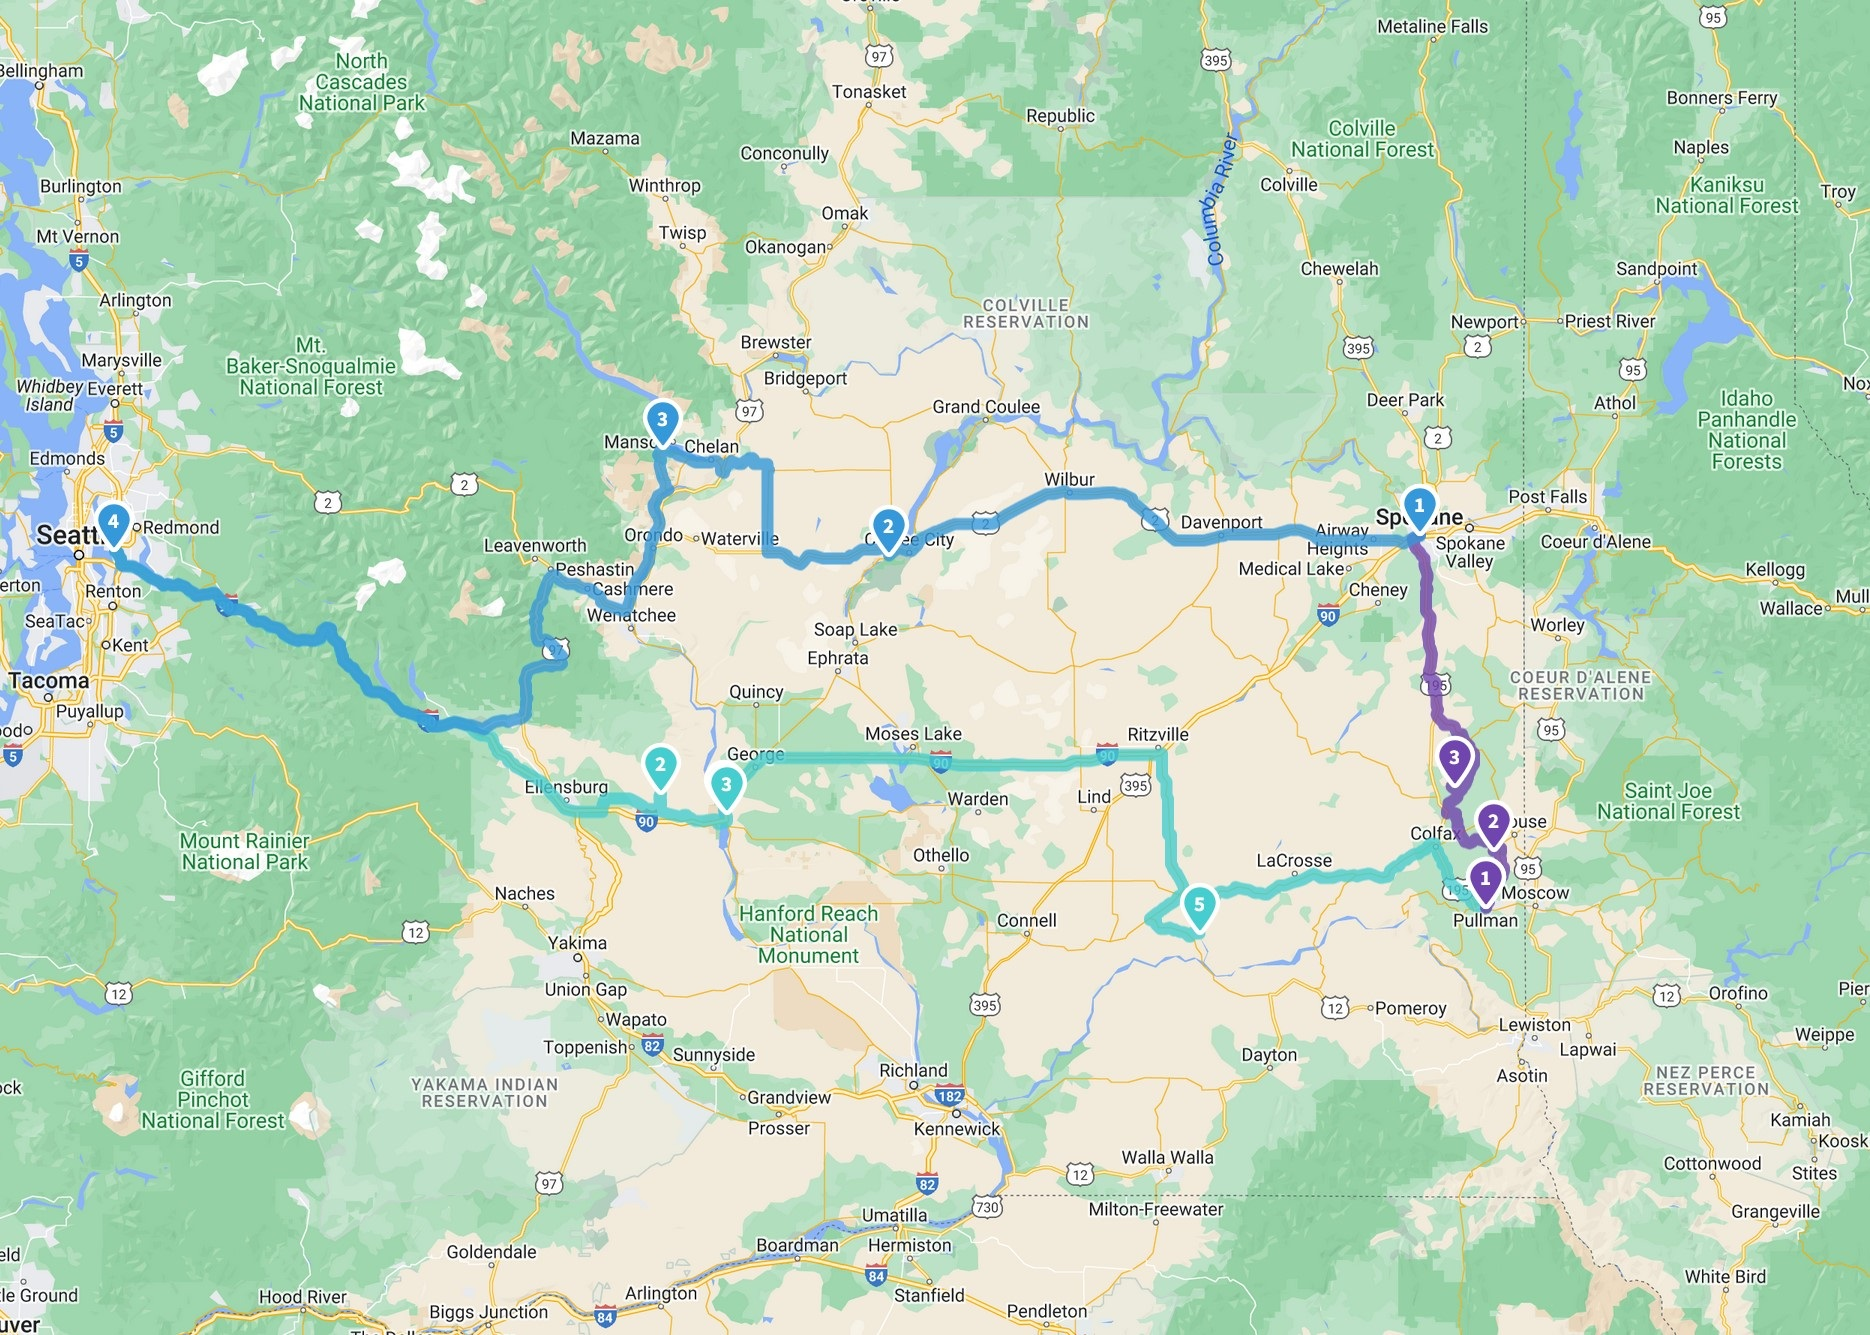
\includegraphics[width=1.3\textwidth]{background.jpg}}; % Change "example-image.jpg" to the filename of your JPEG image

      % Timneline
      % \draw[timeline] (1.1,\DayOneTimelineY) -- (\DayTwoTimelineX, \DayOneTimelineY);

      % Bellevue Square
      \draw[myline] (\DayOnePOneX,0.5) -- (\DayOnePOneX,7.8);

      \draw[<->,myline] (\DayOnePOneX,\DayOneTimelineY) -- (\DayOnePTwoX,\DayOneTimelineY) node[midway,durationText] {2.5 hours};
      \node[timelineText] at (\DayOnePOneX,\DayOneYOne) {08:00};

      % Wild Horse Renewable Energy Center
      \draw[linkingLineDayOne] (\DayOnePTwoX,0.5) -- (\DayOnePTwoX,\DayOneTimelineY) -- (\DayOnePTwoX,4.1) -- (6.5,5.3);
      \node[locationTextDayOne] at (\DayOnePTwoX,4.1) {\WildHorseRenewableEnergyCenter};

      \draw[<->,myline] (\DayOnePTwoX,\DayOneTimelineY) -- (\DayOnePThreeX,\DayOneTimelineY) node[midway,durationText] {1 hour};
      \node[timelineText] at (\DayOnePTwoX,\DayOneYOne) {10:30-11:00};

      % Wild Horse Monument
      % Scenic Overlook of the Columbia River
      \draw[linkingLineDayOne] (\DayOnePThreeX,0.5) -- (\DayOnePThreeX,\DayOneTimelineY) -- (\DayOnePThreeX,2.3) -- (7.15,5.1);
      \node[locationTextDayOne] at (\DayOnePThreeX,2.3) {\WildHorseMonument \\ \ScenicOverlookOftheColumbiaRiver};

      \draw[<->,myline] (\DayOnePThreeX,\DayOneTimelineY) -- (\DayOnePFourX,\DayOneTimelineY) node[midway,durationText] {2 hours};
      \node[timelineText] at (\DayOnePThreeX,\DayOneYOne) {12:00-14:00};

      % Palouse Falls State Park
      \draw[linkingLineDayOne] (\DayOnePFourX,0.5) -- (\DayOnePFourX,\DayOneTimelineY) -- (\DayOnePFourX,3.5) -- (11.79,4.0);
      \node[locationTextDayOne] at (\DayOnePFourX,3.5) {\PalouseFallsStatePark};

      \draw[<->,myline] (\DayOnePFourX,\DayOneTimelineY) -- (\DayTwoTimelineX,\DayOneTimelineY) node[midway,durationText] {2 hours};
      \node[timelineText] at (\DayOnePFourX,\DayOneYOne) {16:00-17:30};

      % Pullman
      \draw[linkingLineDayTwo] (\DayTwoTimelineX,0.5) -- (\DayTwoTimelineX,\DayOneTimelineY) -- (14.6,2.5) -- (14.6,4.2);
      \node[timelineText] at (\DayTwoTimelineX,\DayOneYOne) {19:30 \Pullman};

      % Dots
      \filldraw[timelineDotFill] (\DayOnePOneX,\DayOneTimelineY) circle [timelineCircle];
      \filldraw[timelineDotFillDayOne] (\DayOnePTwoX,\DayOneTimelineY) circle [timelineCircle];
      \filldraw[timelineDotFillDayOne] (\DayOnePThreeX,\DayOneTimelineY) circle [timelineCircle];
      \filldraw[timelineDotFillDayOne] (\DayOnePFourX,\DayOneTimelineY) circle [timelineCircle];
      \filldraw[timelineDotFill] (\DayTwoTimelineX,\DayOneTimelineY) circle [timelineCircle];


      % Day 2
      % Timneline
      % \draw[timeline] (\DayTwoTimelineX,\DayTwoPOneY) -- (\DayTwoTimelineX,\DayTwoPTwoY) -- (\DayTwoTimelineX,\DayTwoPThreeY) -- (\DayTwoTimelineX,\DayTwoPFourY);

      \draw[myline] (\DayTwoXOne,\DayTwoPOneY) -- (\DayTwoTimelineX,\DayTwoPOneY);
      
      % Kamiak Butte Country Park
      \draw[linkingLineDayTwo] (\DayTwoXOne,\DayTwoPTwoY) -- (\DayTwoTimelineX,\DayTwoPTwoY) -- (14.7,5.0);
      \node[locationTextDayTwo] at (\DayTwoTimelineX-4.0,\DayTwoPTwoY) {\KamiakButteCountryPark};

      % Steptoe Butte State Park
      \draw[linkingLineDayTwo] (\DayTwoXOne,\DayTwoPThreeY) -- (\DayTwoTimelineX,\DayTwoPThreeY) -- (\DayTwoTimelineX-1,\DayTwoPThreeY) -- (14.3,5.8);
      \node[locationTextDayTwo] at (\DayTwoTimelineX-2.8,\DayTwoPTwoY+1.6) {\SteptoeButteStatePark};

      % Spokane
      \draw[linkingLineDayThree] (\DayTwoXOne,\DayTwoPFourY) -- (\DayTwoTimelineX,\DayTwoPFourY) -- (13.90,10) -- (13.90,8.35);

      % timeline dots
      \draw[<->,myline] (\DayTwoTimelineX,\DayTwoPOneY) -- (\DayTwoTimelineX,\DayTwoPTwoY) node[midway,right,durationText] {0.5 hours};
      \draw[<->,myline] (\DayTwoTimelineX,\DayTwoPTwoY) -- (\DayTwoTimelineX,\DayTwoPThreeY) node[midway,right,durationText] {45 minutes};
      \draw[<->,myline] (\DayTwoTimelineX,\DayTwoPThreeY) -- (\DayTwoTimelineX,\DayTwoPFourY)node[midway,right,durationText] {1.5 hours};

      \filldraw[timelineDotFill] (\DayTwoTimelineX,\DayTwoPOneY) circle [timelineCircle];
      \filldraw[timelineDotFillDayTwo] (\DayTwoTimelineX,\DayTwoPTwoY) circle [timelineCircle];
      \filldraw[timelineDotFillDayTwo] (\DayTwoTimelineX,\DayTwoPThreeY) circle [timelineCircle];
      \filldraw[timelineDotFill] (\DayTwoTimelineX,\DayTwoPFourY) circle [timelineCircle];

      \node[timelineText] at (\DayTwoXOne-0.5,\DayTwoPOneY) {09:00};
      \node[timelineText] at (\DayTwoXOne-0.5,\DayTwoPTwoY) {09:30-10:30};
      \node[timelineText] at (\DayTwoXOne-0.5,\DayTwoPThreeY) {11:30-12:30};
      \node[timelineText] at (\DayTwoXOne-0.5,\DayTwoPFourY) {14:00 \Spokane};

      % Day 3
      % Timneline
      % \draw[timeline] (\DayThreePOneX,\DayThreeTimelineY) -- (\DayThreePFourX,\DayThreeTimelineY);

      \draw[myline] (\DayThreePOneX,\DayThreeYOne) -- (\DayThreePOneX,\DayThreeTimelineY);

      % Dry Falls Visitor Center
      \draw[linkingLineDayThree] (\DayThreePTwoX,\DayThreeYOne) -- (\DayThreePTwoX,\DayThreeTimelineY) -- (\DayThreePTwoX,\DayThreeTimelineY-3.0) -- (8.8,8.1);
      \node[locationTextDayThree] at (\DayThreePTwoX,\DayThreeTimelineY-3.0) {\DryFallsVisitorCenter};

      % Lake Chelan State Park
      \draw[linkingLineDayThree] (\DayThreePThreeX,\DayThreeYOne) -- (\DayThreePThreeX,\DayThreeTimelineY) -- (\DayThreePThreeX,\DayThreeTimelineY-2) -- (6.4,9.2);
      \node[locationTextDayThree] at (\DayThreePThreeX,\DayThreeTimelineY-2) {\LakeChelanStatePark};

      % Bellevue Square
      \draw[myline] (\DayThreePFourX,\DayThreeYOne) -- (\DayThreePFourX,\DayThreeTimelineY) -- (\DayOnePOneX,7.8);

      % timeline dots
      \draw[<->,myline] (\DayThreePOneX,\DayThreeTimelineY) -- (\DayThreePTwoX,\DayThreeTimelineY) node[midway,durationText] {2 hours};
      \draw[<->,myline] (\DayThreePTwoX,\DayThreeTimelineY) -- (\DayThreePThreeX,\DayThreeTimelineY) node[midway,durationText] {2.5 hours};
      \draw[<->,myline] (\DayThreePThreeX,\DayThreeTimelineY) -- (\DayThreePFourX,\DayThreeTimelineY) node[midway,durationText] {4.5 hours};
      \draw[<->,myline] (\DayThreePTwoX,\DayThreeTimelineY+0.5) -- (\DayThreePFourX,\DayThreeTimelineY+0.5) node[midway,durationText] {4.0 hours};

      \filldraw[timelineDotFill] (\DayThreePOneX,\DayThreeTimelineY) circle [timelineCircle];
      \filldraw[timelineDotFillDayThree] (\DayThreePTwoX,\DayThreeTimelineY) circle [timelineCircle];
      \filldraw[timelineDotFillDayThree] (\DayThreePThreeX,\DayThreeTimelineY) circle [timelineCircle];
      \filldraw[timelineDotFill] (\DayThreePFourX,\DayThreeTimelineY) circle [timelineCircle];

      \node[timelineText] at (\DayThreePOneX,\DayThreeYOne) {09:00};
      \node[timelineText] at (\DayThreePTwoX,\DayThreeYOne) {11:00-12:00};
      \node[timelineText] at (\DayThreePFourX,\DayThreeYOne) {16:00};

    % Draw a circle on the image
    % \draw[red,ultra thick] (3,2) circle (0.5);

    \end{tikzpicture}
    % \caption{Trip to East Washington}
    % \label{fig:image_diagrams}
  \end{figure}

\end{landscape}

\maketitle

% Abstraction
% \begin{abstract}
% 
% This doc presents a three-day travel itinerary for exploring the natural wonders of Eastern Washington.
% The journey encompasses a range of breathtaking landscapes, from the Columbia River to the serene beauty of Lake Chelan.
% Each day is planned to optimize time and provide travelers with an enriching and unforgettable experience.
% The itinerary includes visits to iconic sites such as Palouse Falls State Park, Steptoe Butte State Park, and Dry Falls Visitor Center, among others.
% By following this itinerary, travelers can immerse themselves in the unique and diverse natural landscapes that Eastern Washington has to offer.
% 
% \emph{Keywords}: Travel itinerary, Eastern Washington, natural wonders, Palouse Falls, Lake Chelan, scenic overlooks
% 
% \end{abstract}

% Info
\section{Basic Information}

Travel Date: 05/18/2024(Sat.) - 05/20/2024 (Mon.) \\
Travelers: P1, P2, P3, unknown.

% Preparation
\section{Preparation}
\subsection{Accommodation for Day 1 and Day2 (TBD)}

\begin{itemize}
  \item{Day 1 in \Pullman}
  \begin{itemize}
    \item{\textbf{*AirBnb: \href{https://www.airbnb.com/rooms/38524859?adults=3&check_in=2024-05-18&check_out=2024-05-19}{Charming Condo in Quiet Neighborhood}, \href{https://maps.app.goo.gl/FeBiBENJo8RmT77B7}{Location on Map}}}
    \item{\href{https://maps.app.goo.gl/EwDjgqSxP142zTK69}{\sout{Residence Inn by Marriott Pullman}}}
    \item{\href{https://maps.app.goo.gl/W1NdB4NeXamTnb2G7}{\sout{Coast Hilltop Inn}}}
    \item{AirBnb: \href{https://www.airbnb.com/rooms/959047415867256733?adults=3&check_in=2024-05-18&check_out=2024-05-19}{\sout{Camp Palousa}}}
    \item{...}
  \end{itemize}
  \item{Day 2 in Spokane (or somewhere between \Spokane and \DryFallsVisitorCenter)}
  \begin{itemize}
    \item{\textbf{*AirBnB: \href{https://www.airbnb.com/rooms/630734250409085676?adults=3&check_in=2024-05-19&check_out=2024-05-20}{Cozy Boho Home w/King \& Queen bed}, \href{https://maps.app.goo.gl/bG2gE9wyuAM1cKMC9}{Location on Map}}}
    \item{AirBnB: \href{https://www.airbnb.com/rooms/550276139410529621?adults=3&check_in=2024-05-19&check_out=2024-05-20}{\sout{New 2 Bed 2 Bath Near Perry District and DT!}}}
    \item{AirBnB: \href{https://www.airbnb.com/rooms/802449944852130564?adults=3&check_in=2024-05-19&check_out=2024-05-20}{\sout{Cozy place away from home (3 bedrooms).}}}
    \item{AirBnB: \href{https://www.airbnb.com/rooms/619084546453426629?adults=3&check_in=2024-05-19&check_out=2024-05-20}{\sout{Gorgeous 3 Bedroom Centrally Located Spokane Home}}}
    \item{AirBnb: \href{https://www.airbnb.com/rooms/908205972491427939?adults=3&check_in=2024-05-19&check_out=2024-05-20}{\sout{Renovated 2 bed, 2 bath, Near Arena and Downtown}}, \href{https://maps.app.goo.gl/YyZHSUGSai8nPxxVA}{Location on Map}}
    \item{\href{https://maps.app.goo.gl/q4VfxJgmbbmMeNXL6}{The Davenport Lusso, Autograph Collection}}
    \item{\href{https://maps.app.goo.gl/Ca7z3rT2maDN9GnBA}{Hampton Inn Spokane}}
    \item{...}
  \end{itemize}
\end{itemize}

\subsection{Before Departure}
\begin{itemize}
  \item{Lunch for Day 1.}
  \item{Fruits, snacks}
  \item{...}
\end{itemize}

% Day 1
\section{Day 1}
  \begin{figure}[H]
    \centering
    \begin{tikzpicture}[
      node distance=0.6cm,
      start chain=firstchain going right,
      box/.style={draw, rectangle, minimum width=2cm, minimum height=0.6cm, on chain}
    ]
    \node[box] (node1) {Bellevue};
    \node[box] (node2) {\WildHorseRenewableEnergyCenter};
    \node[box] (node3) {\WildHorseMonument};

    % Automatically wrap the chain if it exceeds the available width
    \begin{scope}[start chain=secondchain going below, node distance=0.6cm, every node/.append style={on chain=secondchain}]
      \node[box, below=of firstchain-end] (node4) {\ScenicOverlookOftheColumbiaRiver};
    \end{scope}
    \begin{scope}[start chain=thirdchain going left, node distance=0.6cm, every node/.append style={on chain=thirdchain}]
      \node[box, left=of secondchain-end] (node5) {\PalouseFallsStatePark};
      \node[box] (node6) {\Pullman};
    \end{scope}

    % Add arrows between nodes
    \draw[->] (node1) -- (node2);
    \draw[->] (node2) -- (node3);
    \draw[->] (node3) -- (node4);
    \draw[->] (node4) -- (node5);
    \draw[->] (node5) -- (node6);
    \end{tikzpicture}
  \end{figure}

\subsection{\WildHorseRenewableEnergyCenter}
\begin{itemize}
  \item{No hiking}
  \item{siteviewing}
\end{itemize}

  %% \begin{figure}[H]
  %%   \centering
  %%   \begin{tikzpicture}
  %%   % Include the JPEG image
  %%     \node[anchor=south west,inner sep=0,opacity=1,scale=0.5] (image) at (0,0) {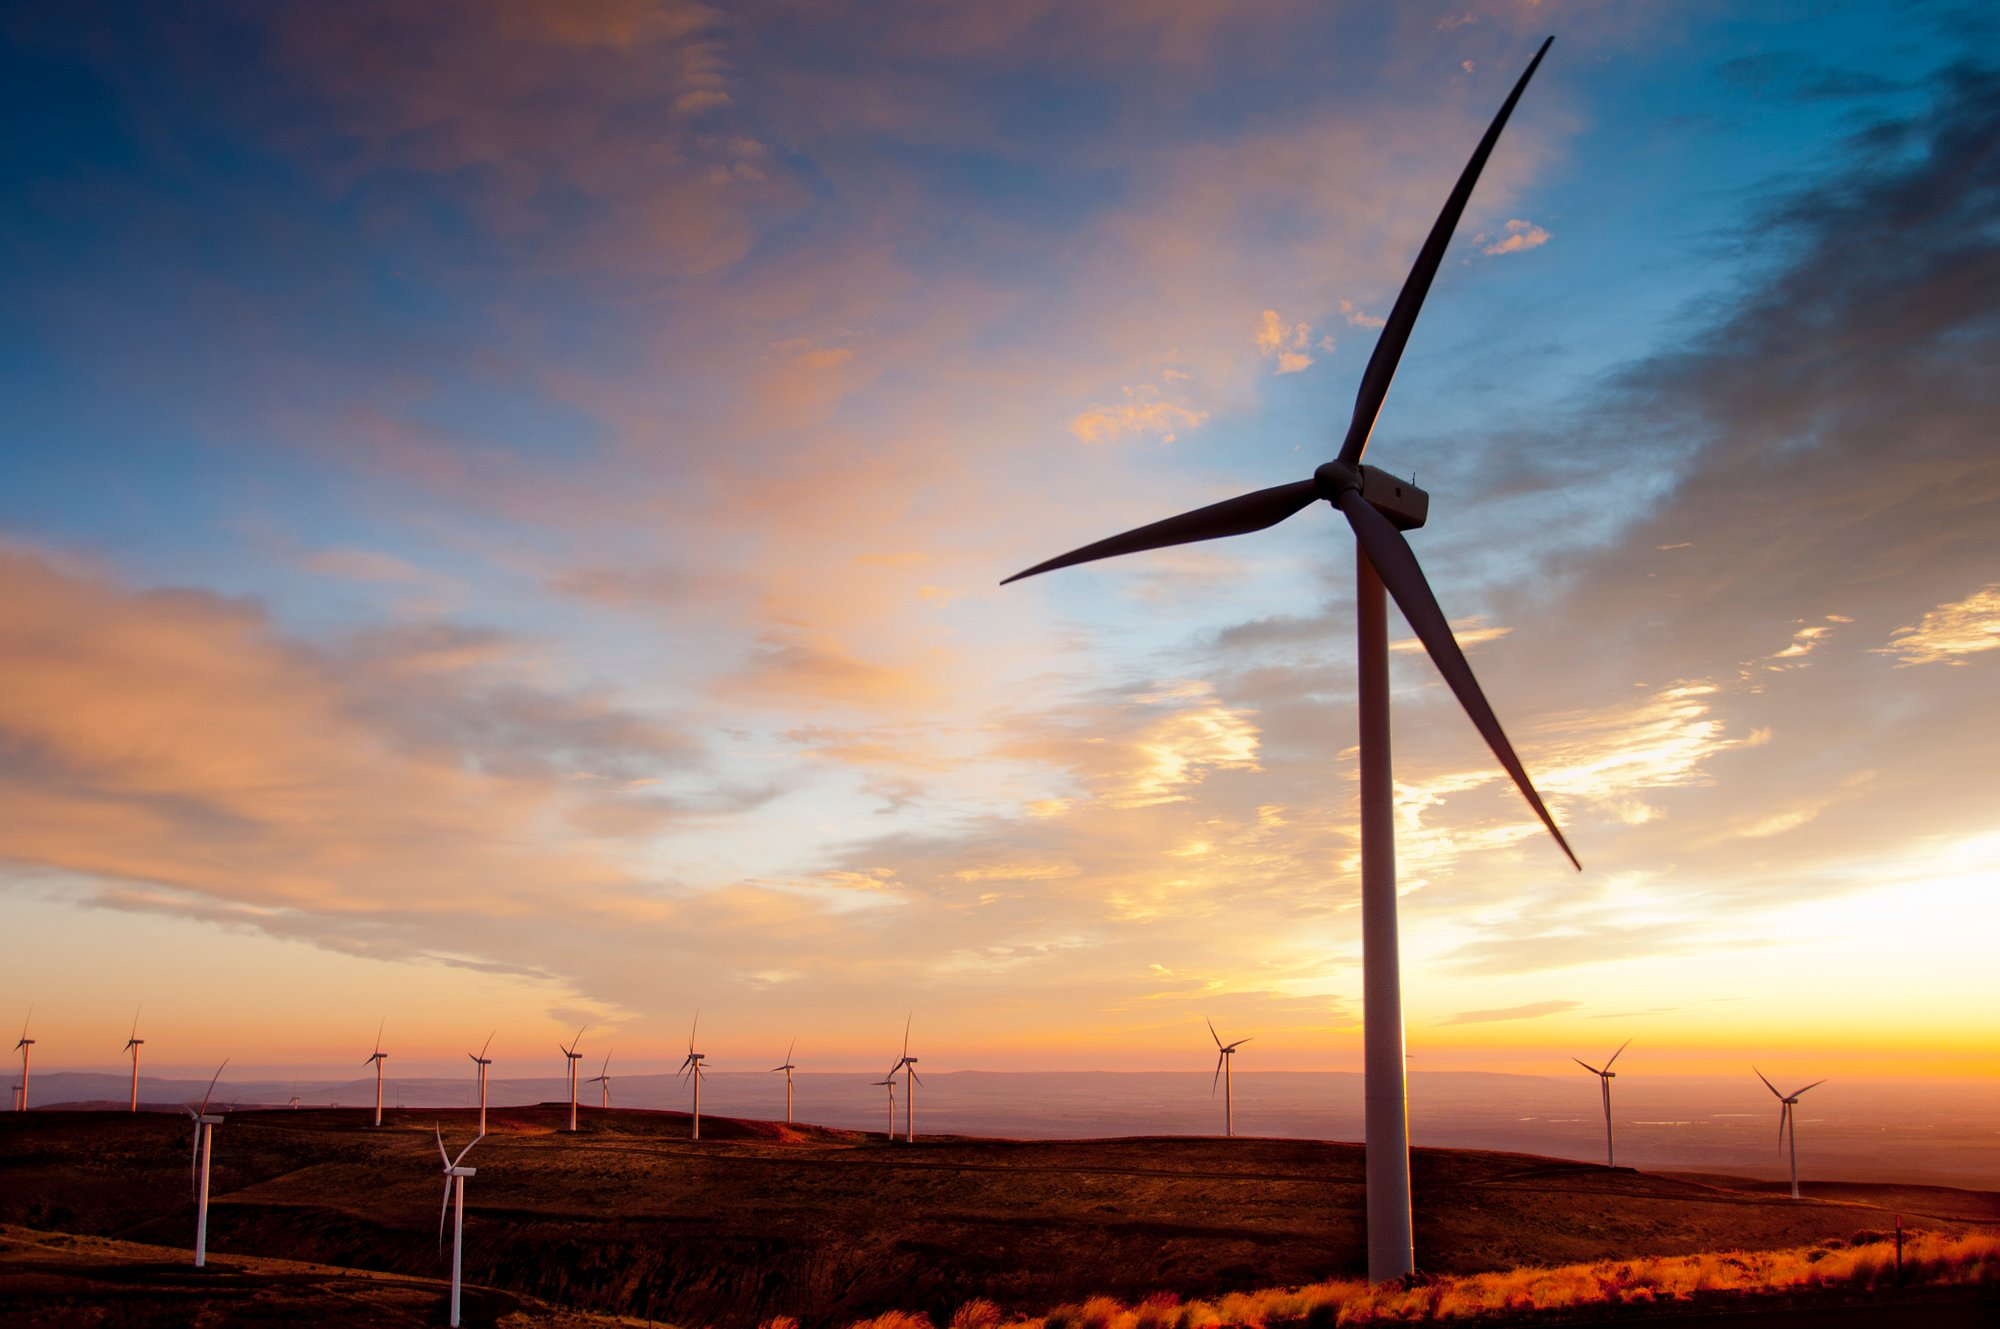
\includegraphics[width=1.3\textwidth]{_images/Wild Horse Renewable Energy Center.jpg}}; % Change "example-image.jpg" to the filename of your JPEG image
  %%   \end{tikzpicture}
  %%   \caption{Wild Horse Renewable Energy Center}
  %% \end{figure}

\subsection{\WildHorseMonument}
\begin{itemize}
  \item{\WildHorseMonumentWebsite}
  \item{View of Columbia River}
  \item{\textit{Enjoy this 0.4-mile out-and-back trail near Beverly, Washington. Generally considered a moderately challenging route, it takes an average of 15 min to complete.
  This trail is great for hiking and walking, and it's unlikely you'll encounter many other people while exploring. The best times to visit this trail are March through July.}}
\end{itemize}

  %% \begin{figure}[H]
  %%   \centering
  %%   \begin{tikzpicture}
  %%   % Include the JPEG image
  %%     \node[anchor=south west,inner sep=0,opacity=1,scale=0.5] (image) at (0,0) {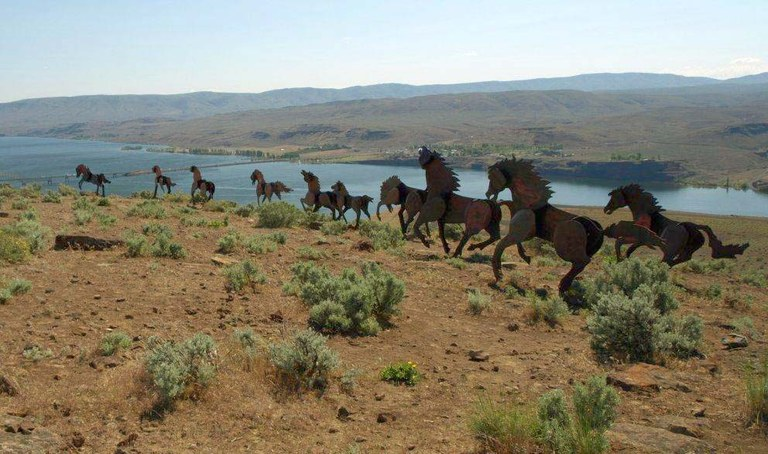
\includegraphics[width=1.3\textwidth]{_images/Wild Horse Monument.jpg}}; % Change "example-image.jpg" to the filename of your JPEG image
  %%   \end{tikzpicture}
  %%   \caption{Wild Horse Monument}
  %% \end{figure}

\subsection{\ScenicOverlookOftheColumbiaRiver}

\begin{itemize}
  \item{Near view of Columbia River}
\end{itemize}

  %% \begin{figure}[H]
  %%   \centering
  %%   \begin{tikzpicture}
  %%   % Include the JPEG image
  %%     \node[anchor=south west,inner sep=0,opacity=1,scale=0.5] (image) at (0,0) {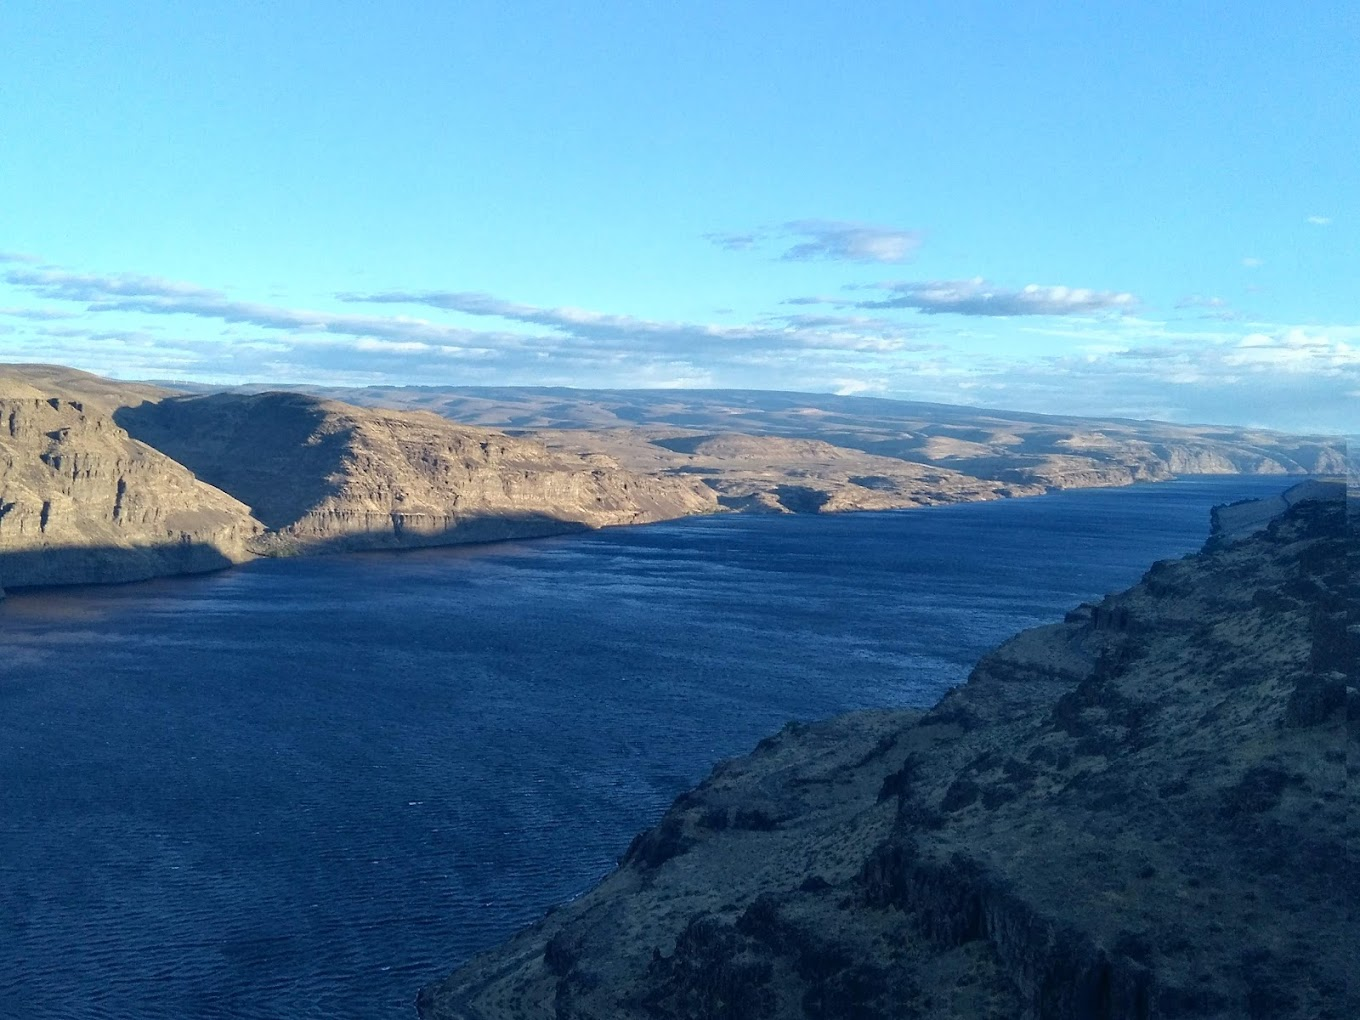
\includegraphics[width=1.3\textwidth]{_images/Scenic Overlook of the Columbia River.jpg}}; % Change "example-image.jpg" to the filename of your JPEG image
  %%   \end{tikzpicture}
  %%   \caption{Scenic Overlook of the Columbia River}
  %% \end{figure}

\subsection{\PalouseFallsStatePark}
\begin{itemize}
  \item{Moderate hiking to the bottom of Palouse Falls}
  \item{\href{https://www.alltrails.com/parks/us/washington/palouse-falls-state-park}{All Trails}}
\end{itemize}
  %% \begin{figure}[H]
  %%   \centering
  %%   \begin{tikzpicture}
  %%   % Include the JPEG image
  %%     \node[anchor=south west,inner sep=0,opacity=1,scale=0.5] (image) at (0,0) {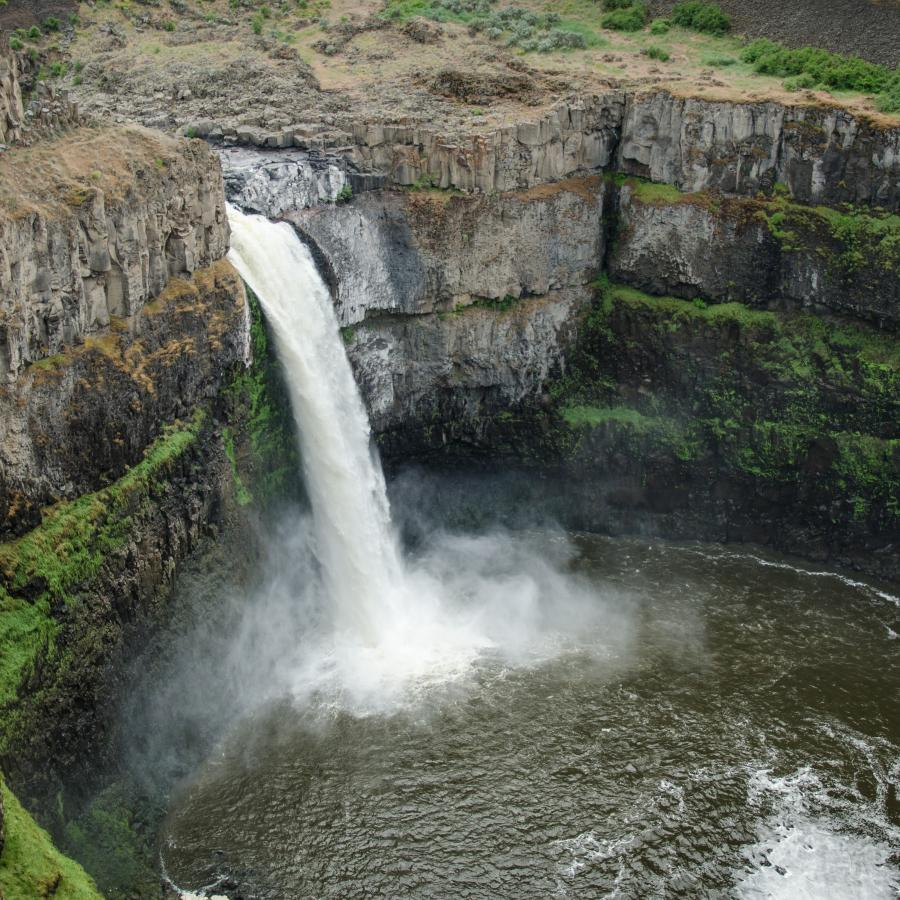
\includegraphics[width=1.3\textwidth]{_images/Palouse Falls State Park.jpg}}; % Change "example-image.jpg" to the filename of your JPEG image
  %%   \end{tikzpicture}
  %%   \caption{Palouse Falls State Park}
  %% \end{figure}

\subsection{Pullman}
\begin{itemize}
  \item{WSU: Washington State University}
\end{itemize}

\subsubsection{Dinner}

% Day 2
\section{Day 2}
  \begin{figure}[H]
    \centering
    \begin{tikzpicture}[
      node distance=0.6cm,
      start chain=firstchain going right,
      box/.style={draw, rectangle, minimum width=2cm, minimum height=0.6cm, on chain}
    ]
    \node[box] (node1) {\Pullman};
    \node[box] (node2) {\KamiakButteCountryPark};
    \node[box] (node3) {\SteptoeButteStatePark};
    \node[box] (node4) {\Spokane};

    % Add arrows between nodes
    \draw[->] (node1) -- (node2);
    \draw[->] (node2) -- (node3);
    \draw[->] (node3) -- (node4);
    \end{tikzpicture}
  \end{figure}


\subsection{\KamiakButteCountryPark}
\href{https://www.whitmancounty.org/facilities/facility/details/Kamiak-Butte-County-Park-1}{Kamiak Butte Country Park Website}

\begin{itemize}
  \item{Pine Ridge trail, a 3.5 mile loop, 1.5 hours (Optional). \href{https://www.alltrails.com/trail/us/washington/kamiak-butte-trail}{All Trails}}
\end{itemize}

  %% \begin{figure}[H]
  %%   \centering
  %%   \begin{tikzpicture}
  %%   % Include the JPEG image
  %%     \node[anchor=south west,inner sep=0,opacity=1,scale=0.5] (image) at (0,0) {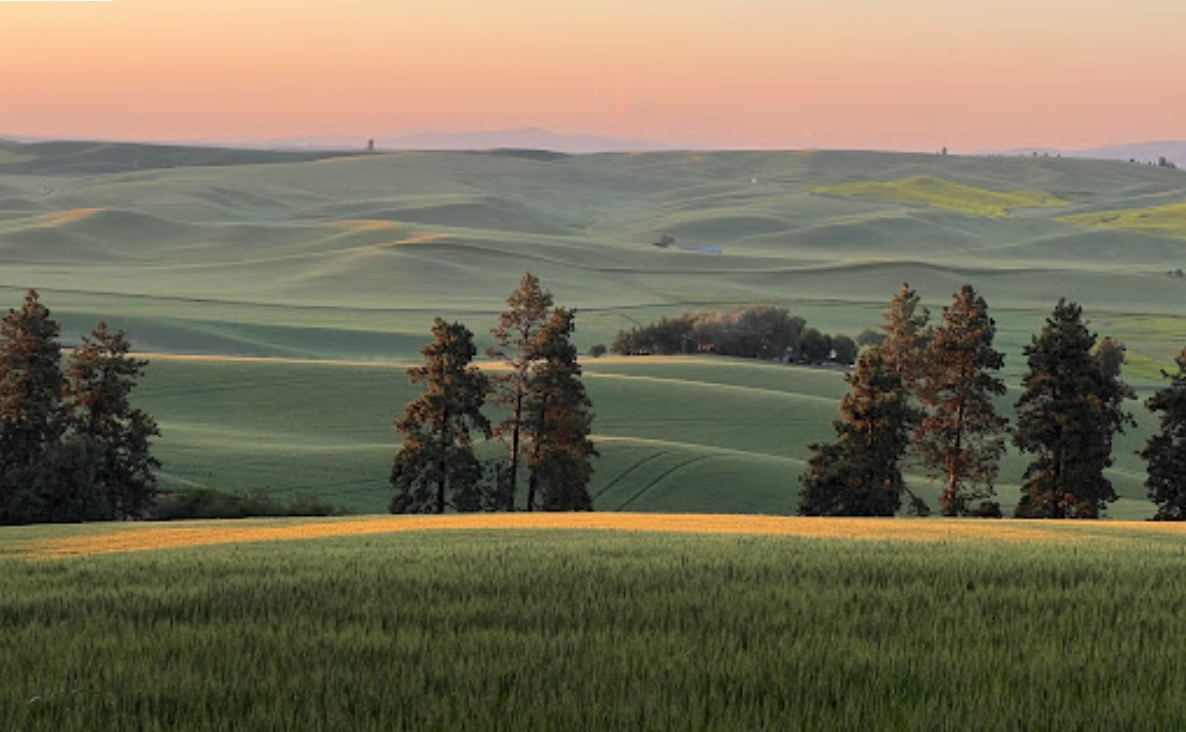
\includegraphics[width=1.3\textwidth]{_images/Kamiak Butte Country Park.jpg}}; % Change "example-image.jpg" to the filename of your JPEG image
  %%   \end{tikzpicture}
  %%   \caption{Kamiak Butte Country Park}
  %% \end{figure}

\subsection{Lunch at \href{https://maps.app.goo.gl/bh54WPhsrkuKu8Ae8}{Colfax} or skip}

\subsection{\SteptoeButteStatePark}
\begin{itemize}
  \item{No Hiking.}
\end{itemize}

  %% \begin{figure}[H]
  %%   \centering
  %%   \begin{tikzpicture}
  %%   % Include the JPEG image
  %%     \node[anchor=south west,inner sep=0,opacity=1,scale=0.5] (image) at (0,0) {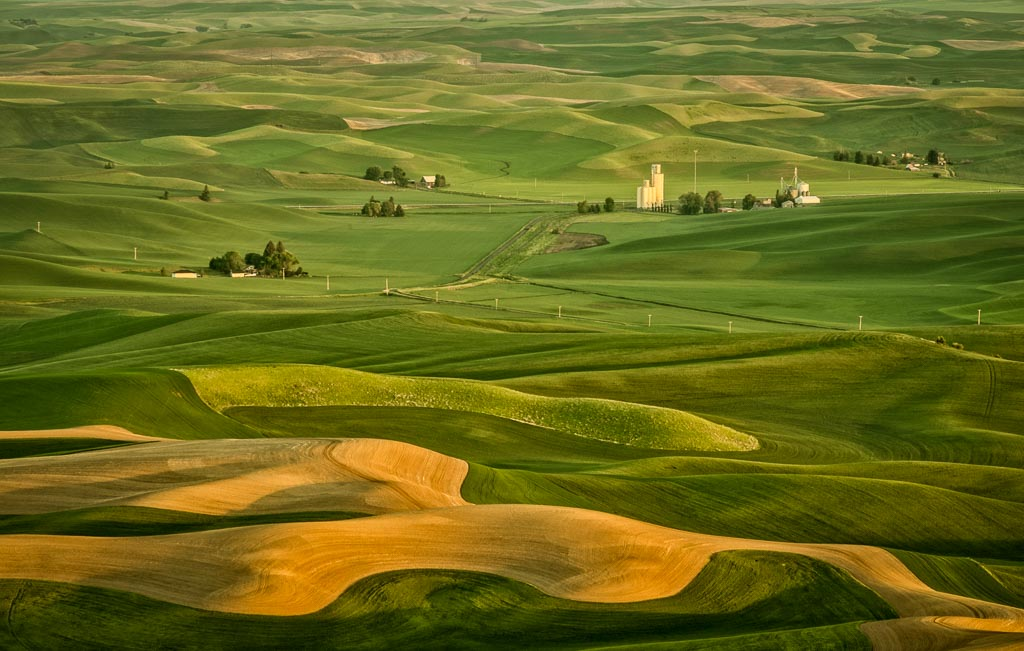
\includegraphics[width=1.3\textwidth]{_images/Steptoe Butte State Park.jpg}}; % Change "example-image.jpg" to the filename of your JPEG image
  %%   \end{tikzpicture}
  %%   \caption{Steptoe Butte State Park}
  %% \end{figure}

\subsection{\Spokane}
Explorer Spokane
\begin{itemize}
  \item{Riverfront Park}
  \begin{itemize}
    \item{\textbf{Spokane Falls (Upper Falls)}}
    \item{\textbf{Spokane Falls (Lower Falls)}}
    \item{Numerica SkyRide}
    \item{Rotary Fountain}
    \item{...}
  \end{itemize}
\end{itemize}

\subsubsection{Dinner}
\begin{itemize}
  \item{\href{https://maps.app.goo.gl/xVXrV7TUJmNi5Nha8}{Vieux Carre NOLA Kitchen}}
  \item{...}
\end{itemize}

% Day 3
\section{Day 3}
  \begin{figure}[H]
    \centering
    \begin{tikzpicture}[
      node distance=0.6cm,
      start chain=firstchain going right,
      box/.style={draw, rectangle, minimum width=2cm, minimum height=0.6cm, on chain}
    ]
    \node[box] (node1) {\Spokane};
    \node[box] (node2) {\DryFallsVisitorCenter};
    \node[box] (node3) {\LakeChelanStatePark};
    \node[box] (node4) {Bellevue};

    % Add arrows between nodes
    \draw[->] (node1) -- (node2);
    \draw[->] (node2) -- (node3);
    \draw[->] (node3) -- (node4);
    \end{tikzpicture}
  \end{figure}
\subsection{\DryFallsVisitorCenter}

  %% \begin{figure}[H]
  %%   \centering
  %%   \begin{tikzpicture}
  %%   % Include the JPEG image
  %%     \node[anchor=south west,inner sep=0,opacity=1,scale=0.5] (image) at (0,0) {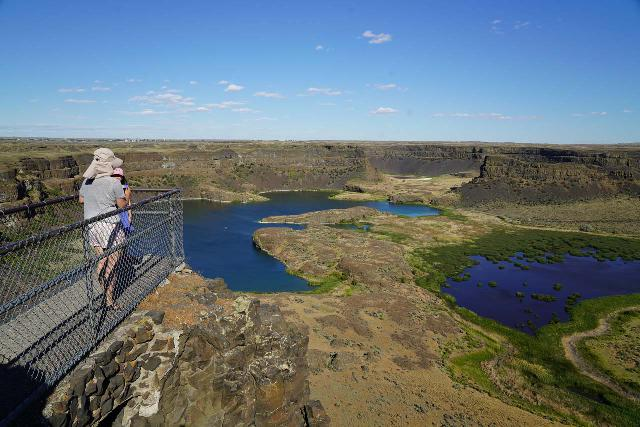
\includegraphics[width=1.3\textwidth]{_images/Dry Falls Visitor Center.jpg}}; % Change "example-image.jpg" to the filename of your JPEG image
  %%   \end{tikzpicture}
  %%   \caption{Dry Falls Visitor Center}
  %% \end{figure}

\subsection{\LakeChelanStatePark}
(May have to skip)
Lake Chelan State Park

\end{document}

